\chapter{Systematic Uncertainties}
\label{chap:syst}

The systematic uncertainties in the signal efficiency is computed by estimating the contribution of each efficiency factor in Eq.~\ref{eq:OverallEff} when possible. 

The systematic uncertainty in track and vertex reconstruction is studied using \Ks in Section~\ref{sec:syst:vertexing}. The systematic uncertainty in trigger is studied in Section~\ref{sec:syst:trigger} using tag-and-probe method with $Z\rightarrow \ee,\mumu$ events. %The systematic uncertainty in lepton reconstruction and identification cannot be estimated using data since no known particle exists in nature that has a long lifetime and mass larger than 10 GeV.



\section{Systematic Uncertainty in Track and Vertex Reconstruction}
\label{sec:syst:vertexing}

In a typical analysis, the systematic uncertainty in track and vertex reconstruction is estimated by the Inner Tracking Combined Performance group using the standard tracking setup. This result cannot be directly used for this analysis due to the special reconstruction setup described in Chapter~\ref{chap:reco}. Instead, the systematic uncertainty in track and vertex reconstruction is estimated by comparing vertex yields between the data and the MC samples using the process, $K_{S}\rightarrow\pi^{+}\pi^{-}$. This process allows the comparison of the efficiencies between data and MC samples to the long lifetime ($c\tau \sim26.8~\si{\mm}$). However, there are intrinsic differences between \Ks and signal long-lived particles such as mass and $p_{T}$. In order to understand the validity and the limitation of this method, the kinematic distributions of \Ks and $Z'$ candidates are compared in Appendix~\ref{app:syst_Ks_Zp}.

Tracks originating from a \Ks decay can be reconstructed by either the standard tracking (ST) or the LRT algorithm, resulting in three categories of \Ks vertices: vertices with two \textit{standard tracks}, one standard track and one \textit{large-radius track}, and two large-radius tracks. \Ks vertex yields in each category can be expressed by total \Ks produced in a sample and tracking and vertexing efficiency,

\begin{align}
    N_{\mathrm{ST}}  &= K_{S}~\mathrm{produced} \times (\epsilon_{\mathrm{ST~Track}})^{2} \cdot \epsilon_{\mathrm{ST~Vertex}}, \nonumber \\
    N_{\mathrm{ST+LRT}}  &= K_{S}~\mathrm{produced} \times (\epsilon_{\mathrm{ST~Track}} \cdot \epsilon_{\mathrm{LRT~Track}}) \cdot \epsilon_{\mathrm{LRT~Vertex}}, \nonumber \\
    N_{\mathrm{LRT}}&= K_{S}~\mathrm{produced} \times (\epsilon_{\mathrm{LRT~Track}})^{2} \cdot \epsilon_{\mathrm{LRT~Vertex}},
\label{eq:Ks_eq1}
\end{align}
%
where $N$ represents vertex yields in each category. $\epsilon_{\mathrm{ST~Track}}$ and $\epsilon_{\mathrm{LRT~Track}}$ represent track reconstruction efficiency in the ST and the LRT, respectively. $\epsilon_{\mathrm{ST~Vertex}}$ and $\epsilon_{\mathrm{LRT~Vertex}}$ represents two-track vertex reconstruction efficiency on two standard or large-radius tracks, respectively.

%In order to compare the efficiency between data and MC samples, the \Ks yields of LRT type in data is normalized by the ratio of ST vertex yields in MC to data,
In order to compare the efficiency between data and MC samples, the \Ks yields of LRT type in data is normalized to the MC for \Ks found with the ST,

\begin{equation}
\mathrm{Normalized~data~to~MC} = \dfrac{N_{\mathrm{LRT}} \cdot \Big(N_{\mathrm{ST}}^{\mathrm{MC}} / N_{\mathrm{ST}}\Big)}{N_{\mathrm{LRT}}^{\mathrm{MC}}},
\label{eq:Ks_eq2}
\end{equation}
%
where quantities estimated using MC samples are denoted by MC, and quantities estimated using data are denoted otherwise. Using Eqs.~\ref{eq:Ks_eq1}$-$~\ref{eq:Ks_eq2}, the systematic uncertainty in track and vertex reconstruction is expressed as,

%\begin{align}
%    \dfrac{\dfrac{N_{LRT}}{N_{ST}}}{\dfrac{N'_{LRT}}{N'_{ST}}}  &= 
%        \dfrac
%        {\dfrac{(\epsilon_{\mathrm{LRT}})^{2} \cdot \epsilon_{\mathrm{LRT~Vertex}}}{(\epsilon_{\mathrm{ST}})^{2} \cdot \epsilon_{\mathrm{ST~Vertex}}}}
%        {\dfrac{(\epsilon'_{\mathrm{LRT}})^{2} \cdot \epsilon'_{\mathrm{LRT~Vertex}}}{(\epsilon'_{\mathrm{ST}})^{2} \cdot \epsilon'_{\mathrm{ST~Vertex}}}}
%\label{eq:Ks_eq2}
%\end{align}

\begin{align}
    \dfrac{N_{\mathrm{LRT}} / N_{\mathrm{ST}}}{N_{\mathrm{LRT}}^{\mathrm{MC}} / N_{\mathrm{ST}}^{\mathrm{MC}}} \cdot &=
    \dfrac{\dfrac{(\epsilon_{\mathrm{LRT~Track}})^{2} \cdot \epsilon_{\mathrm{LRT~Vertex}}}{(\epsilon_{\mathrm{ST~Track}})^{2} \cdot \epsilon_{\mathrm{ST~Vertex}}}}{\dfrac{(\epsilon_{\mathrm{LRT~Track}}^{\mathrm{MC}})^{2} \cdot \epsilon_{\mathrm{LRT~Vertex}}^{\mathrm{MC}}}{(\epsilon_{\mathrm{ST~Track}}^{\mathrm{MC}})^{2} \cdot \epsilon_{\mathrm{ST~Vertex}}^{\mathrm{MC}}}} 
    \\[10pt]
    \Big( \dfrac{\epsilon_{\mathrm{LRT~Track}}}{\epsilon_{\mathrm{LRT~Track}}^{\mathrm{MC}}}\Big)^{2} \cdot
    \Big( \dfrac{\epsilon_{\mathrm{LRT~Vertex}}}{\epsilon_{\mathrm{LRT~Vertex}}^{\mathrm{MC}}}\Big) &=
    \Big( \dfrac{N_{\mathrm{LRT}} \cdot N_{\mathrm{ST}}^{\mathrm{MC}}}{N_{\mathrm{LRT}}^{\mathrm{MC}} \cdot N_{\mathrm{ST}}} \Big) \cdot
    \Big( \dfrac{\epsilon_{\mathrm{ST~Track}}}{\epsilon_{\mathrm{ST~Track}}^{\mathrm{MC}}}\Big)^{2} \cdot
    \Big( \dfrac{\epsilon_{\mathrm{ST~Vertex}}}{\epsilon_{\mathrm{ST~Vertex}}^{\mathrm{MC}}}\Big).
\label{eq:Ks_eq3}
\end{align}

Events are selected using the same event selection described in Section~\ref{sec:selection:pre} except trigger filters as the high-$p_{T}$ photon or muon triggers are not suitable for \Ks study. From the selected events, \Ks candidates, referred as \Ks vertices, are selected by applying \Ks vertex selection to secondary vertices in the events. The \Ks vertex selection is similar to the $Z'$ signal vertex selection, but %for consistency with \Ks study in Run I and 
for background reduction, additional vertex cuts motivated by Ref.~\cite{Oh:1951024} are applied. The mass window of 0.35 to 0.65 GeV is used in the \Ks vertex selection. The difference between \Ks and $Z'$ vertex selections are summarized in Table~\ref{table:ks_vertex_cut}. %Figure~\ref{fig:Ks_vertex_cutflow} shows \Ks vertex cut flow in the data and the background MC samples.

\begin{table}[!htb]
%\begin{table}[tb]
  \centering
  \begin{tabular}{ c c c }
    \hline
    \hline
                    & $Z'$                                                  & \Ks                               \\
    \hline
    Trigger         & Photon or muon trigger (Table~\ref{table:triggers})    & -                                     \\
    Vertex type     & \mumu, \emu, \ee                                      & \xx                                   \\
    Mass (GeV)      & $> 10.0$                                              & $[0.35,0.65]$                         \\
    Additional cut                   & -                                                     & $|\Delta z_{0}| <$ 2 mm               \\
                                     &                                                       & Decay length $>$ 15 mm                \\
    \hline
    \hline
  \end{tabular}
  \caption{Comparison of $Z'$ and \Ks vertex selections.}
  \label{table:ks_vertex_cut}
\end{table}

%\begin{figure}[!htb]
%	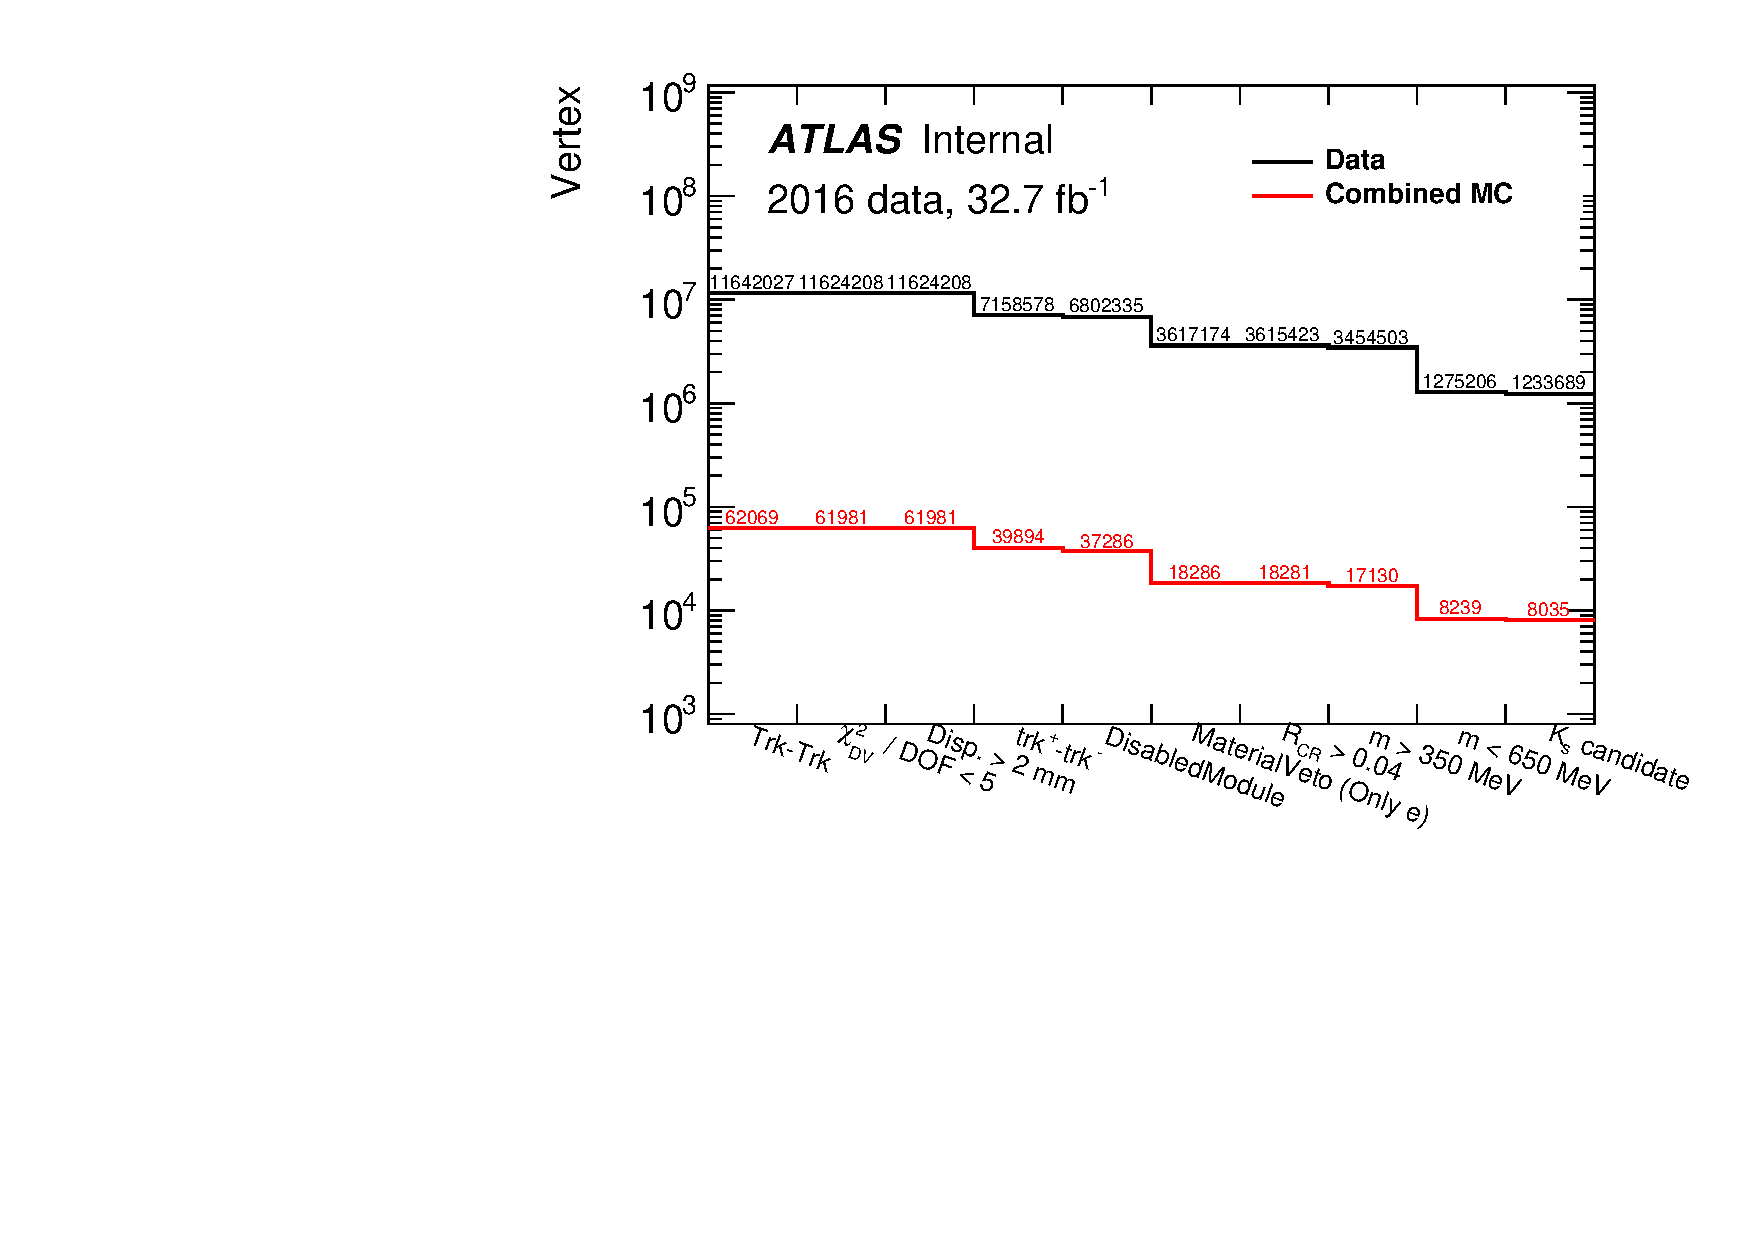
\includegraphics[width=0.60\textwidth]{figures/m_syst_Ks_cf.pdf}
%	\centering
%	\caption{Vertex cut flow applied on \Ks vertices in the data and the MC samples}
%	\label{fig:Ks_vertex_cutflow}
%\end{figure}

After applying the event and \Ks vertex selection, the \Ks vertex distributions in the data and MC samples are compared in Figure~\ref{fig:Ks_data_MC}. The data sample is normalized to the MC samples which have limited statistics. Only \Ks vertices with two large-radius tracks are shown. The distributions show good agreement in the invariant mass, $p_{T}$, transverse and longitudinal position, and decay length of the vertices, except the pile-up distribution as expected.


\begin{figure}[!htb]
    \centering
    \subfloat[]{\label{subfig:Ks_m}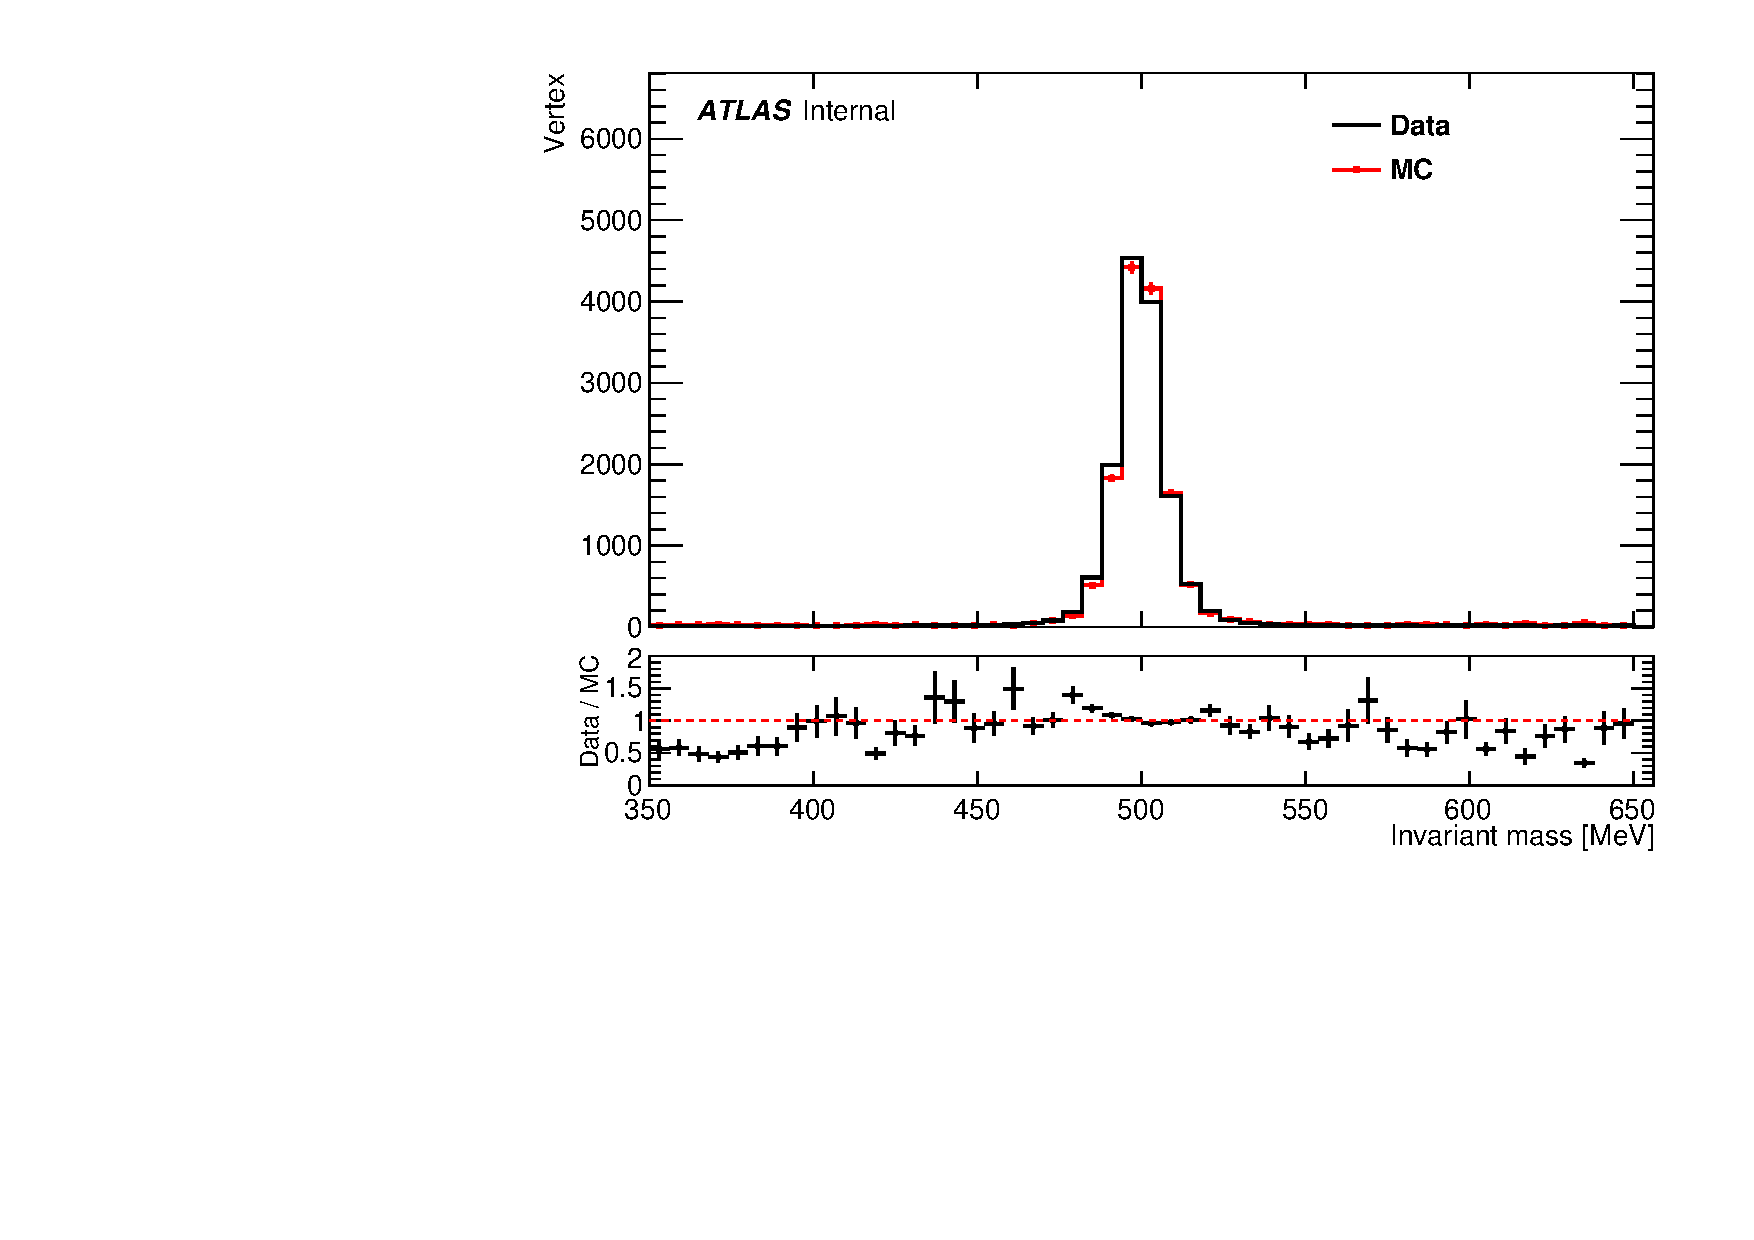
\includegraphics[width=0.45\textwidth]{figures/m_syst_Ks_M.pdf}}
    \subfloat[]{\label{subfig:Ks_pt}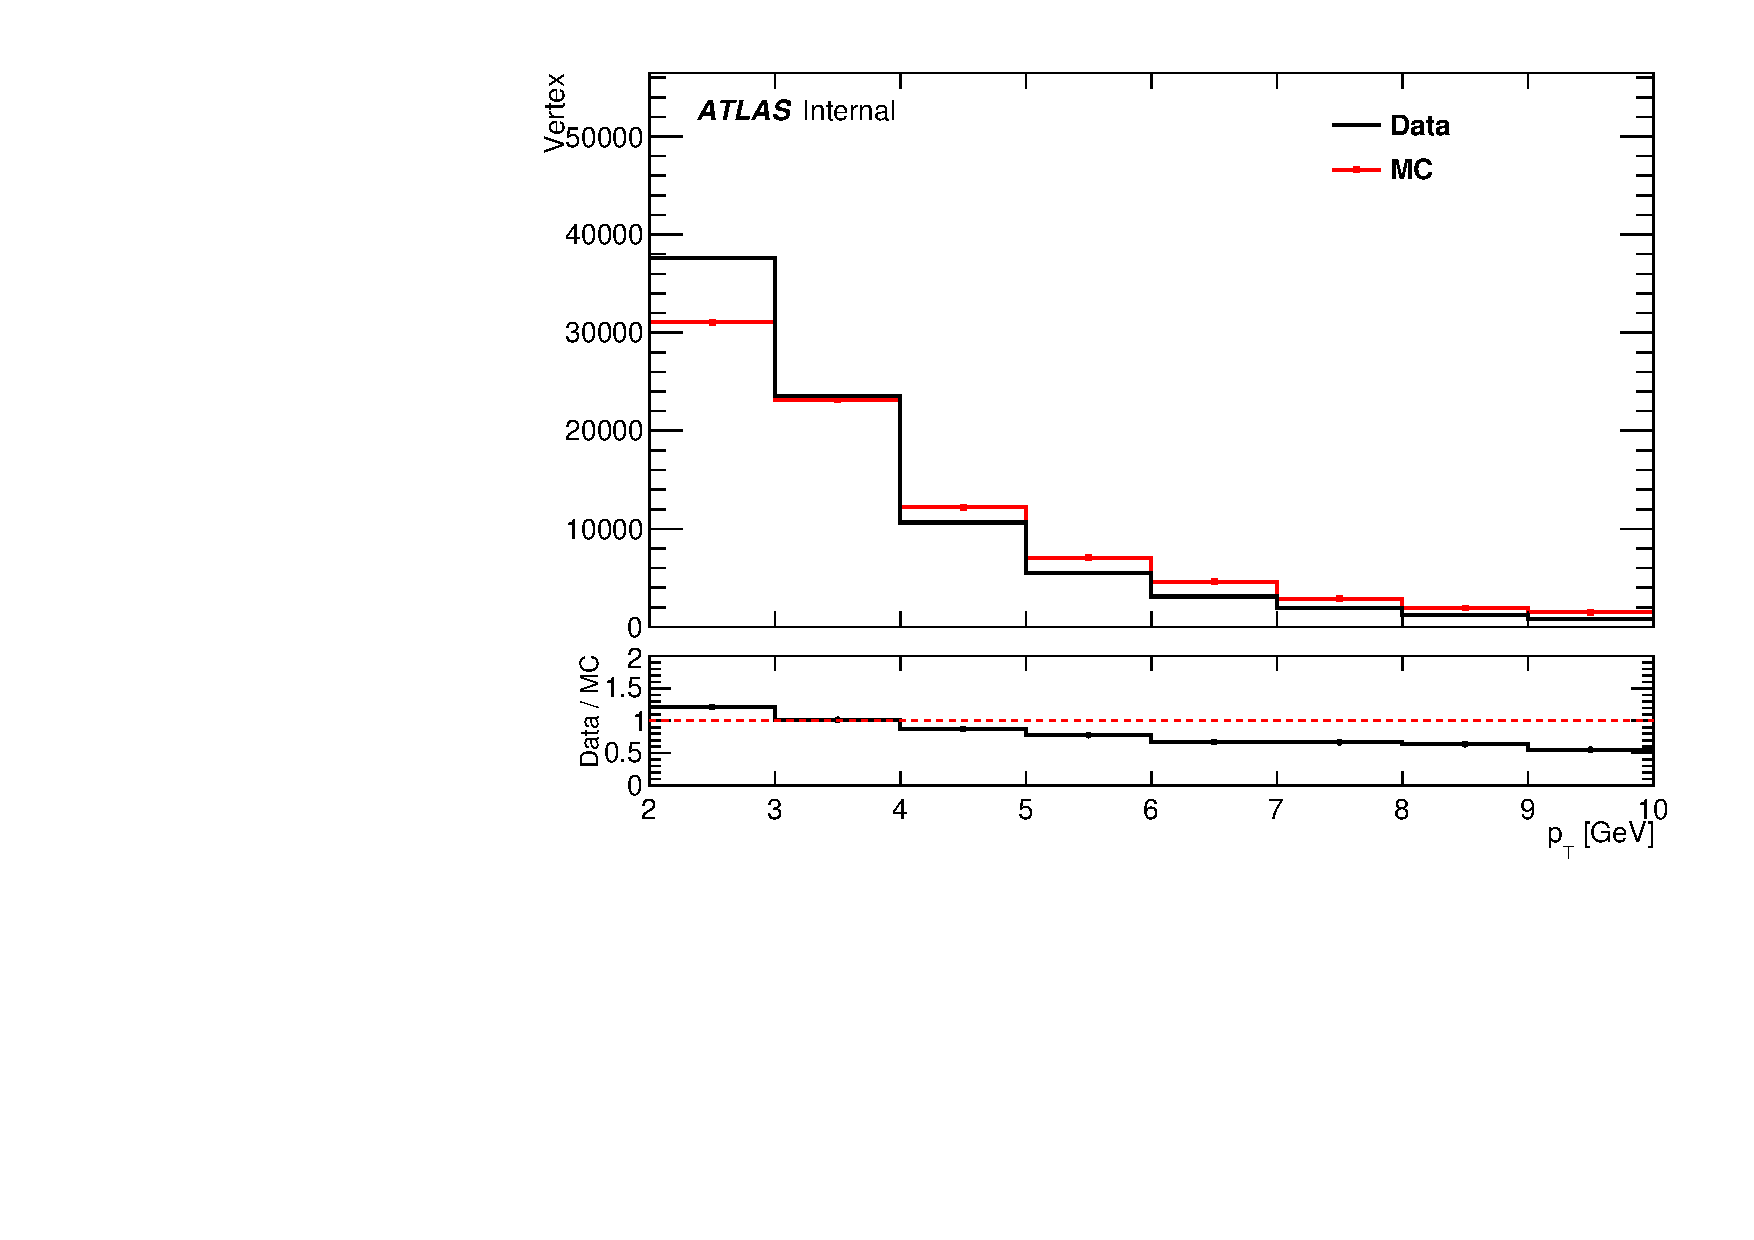
\includegraphics[width=0.45\textwidth]{figures/m_syst_Ks_pt.pdf}} \\
    \subfloat[]{\label{subfig:Ks_mu}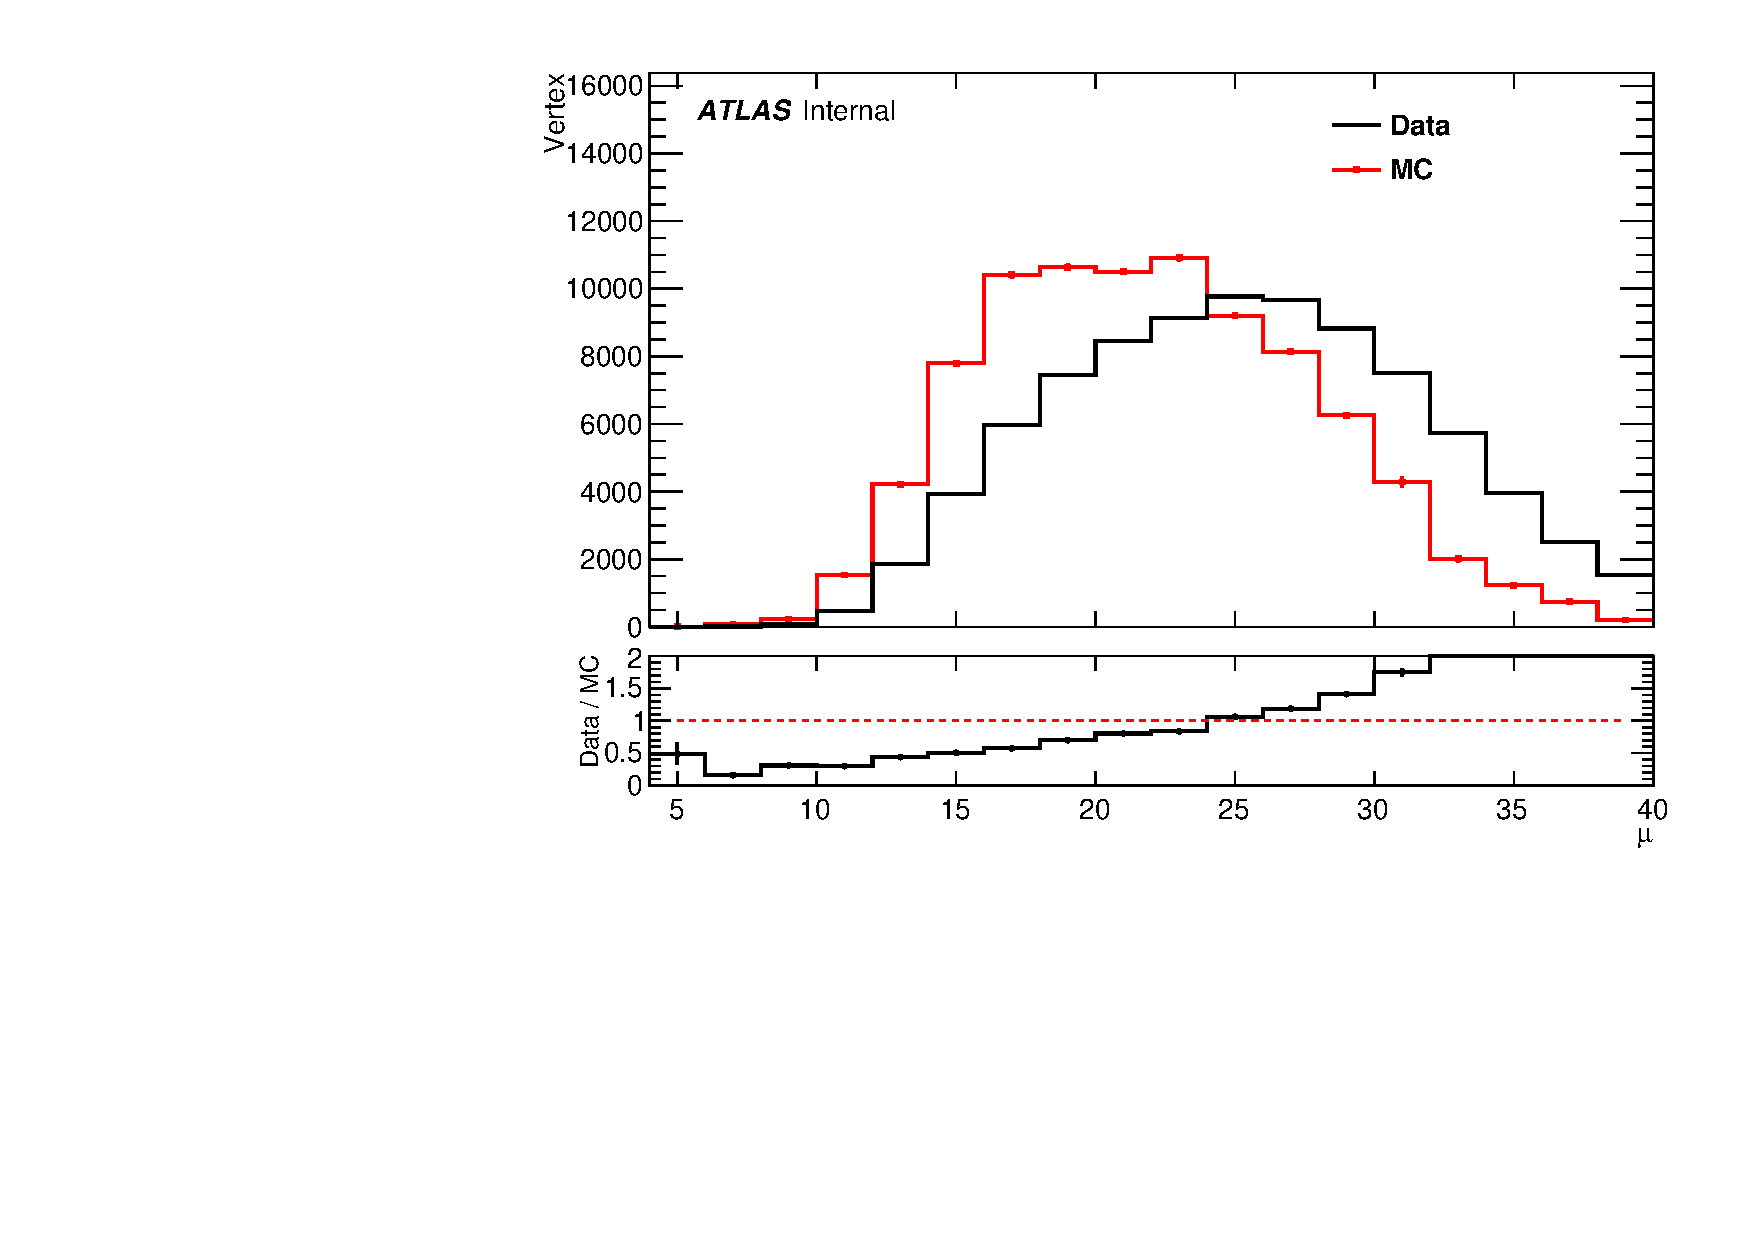
\includegraphics[width=0.45\textwidth]{figures/m_syst_Ks_mu.pdf}}
    \subfloat[]{\label{subfig:Ks_r}\includegraphics[width=0.45\textwidth]{figures/m_syst_Ks_r.pdf}}  \\
    \subfloat[]{\label{subfig:Ks_z}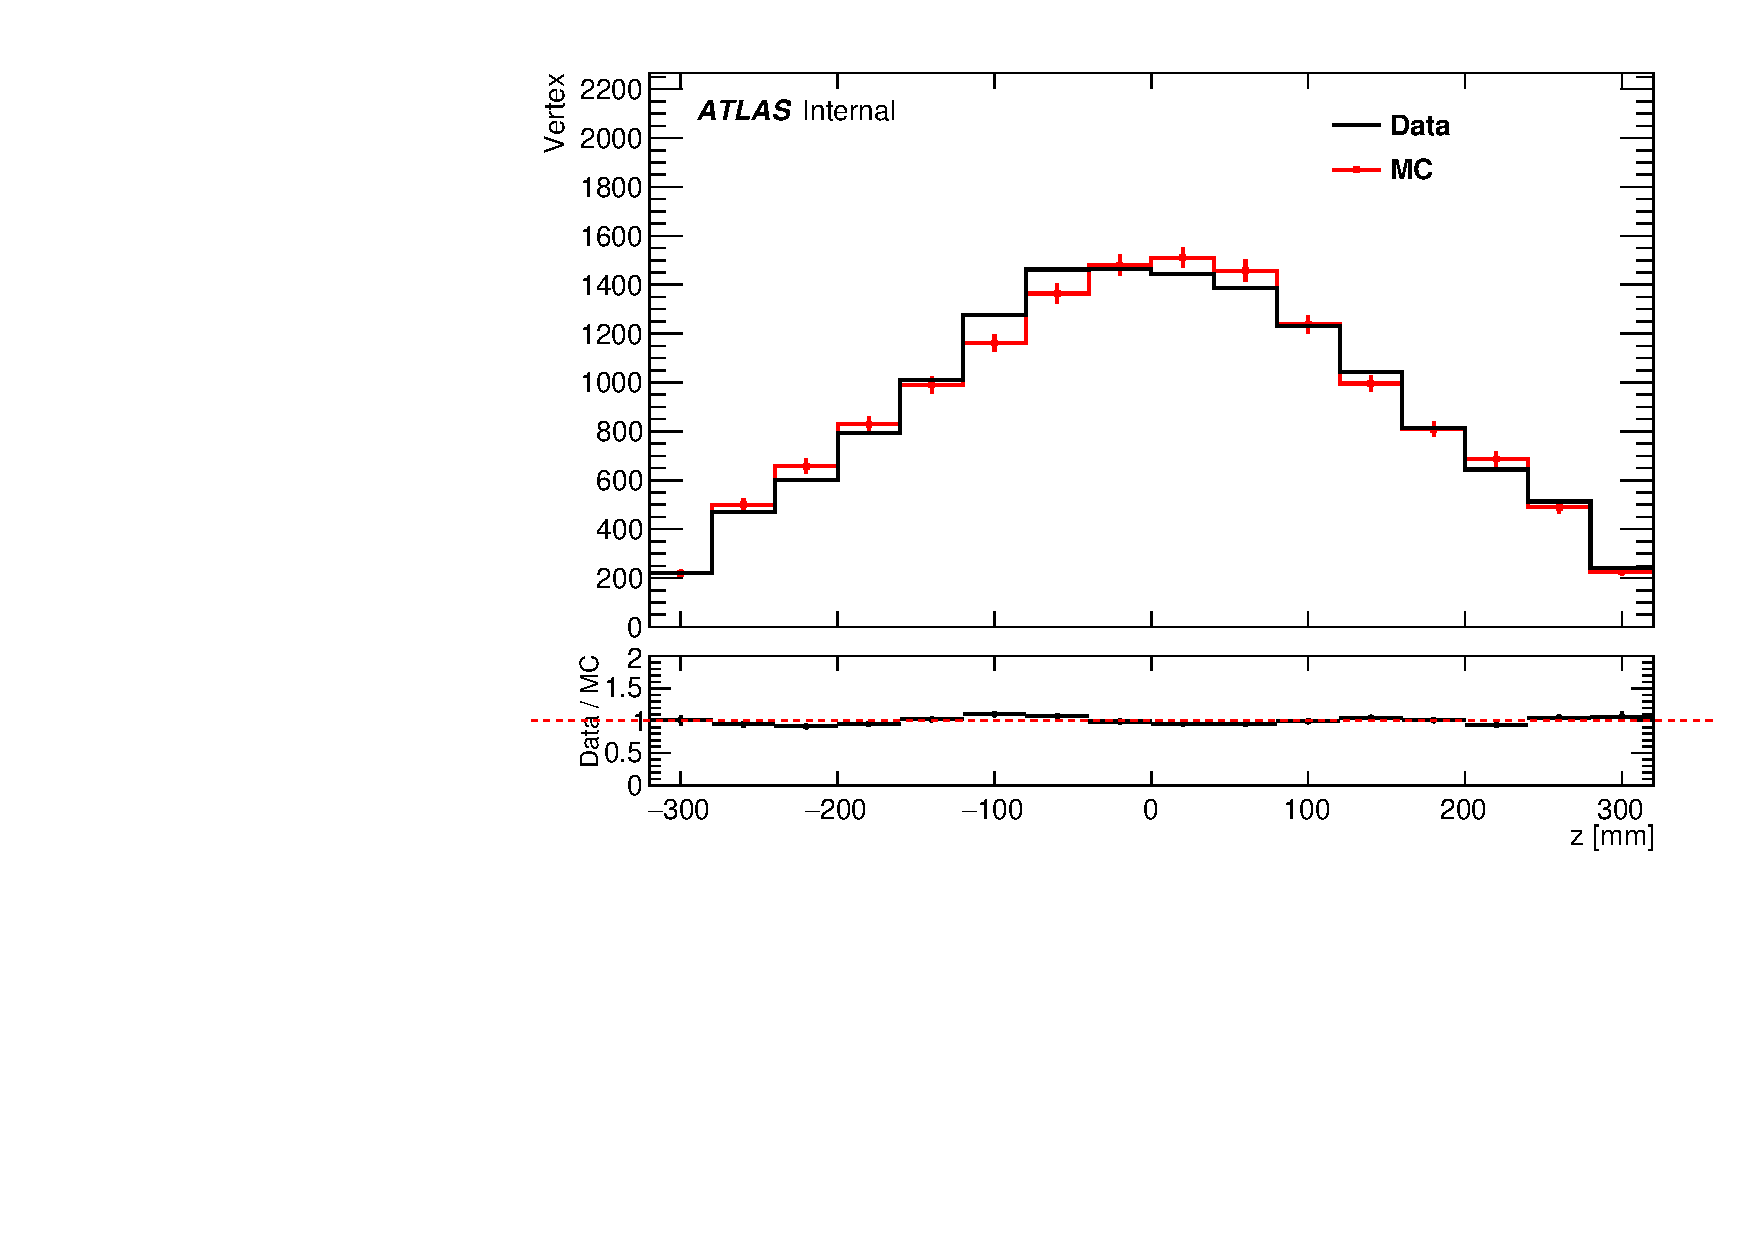
\includegraphics[width=0.45\textwidth]{figures/m_syst_Ks_z.pdf}} 
    \subfloat[]{\label{subfig:Ks_l}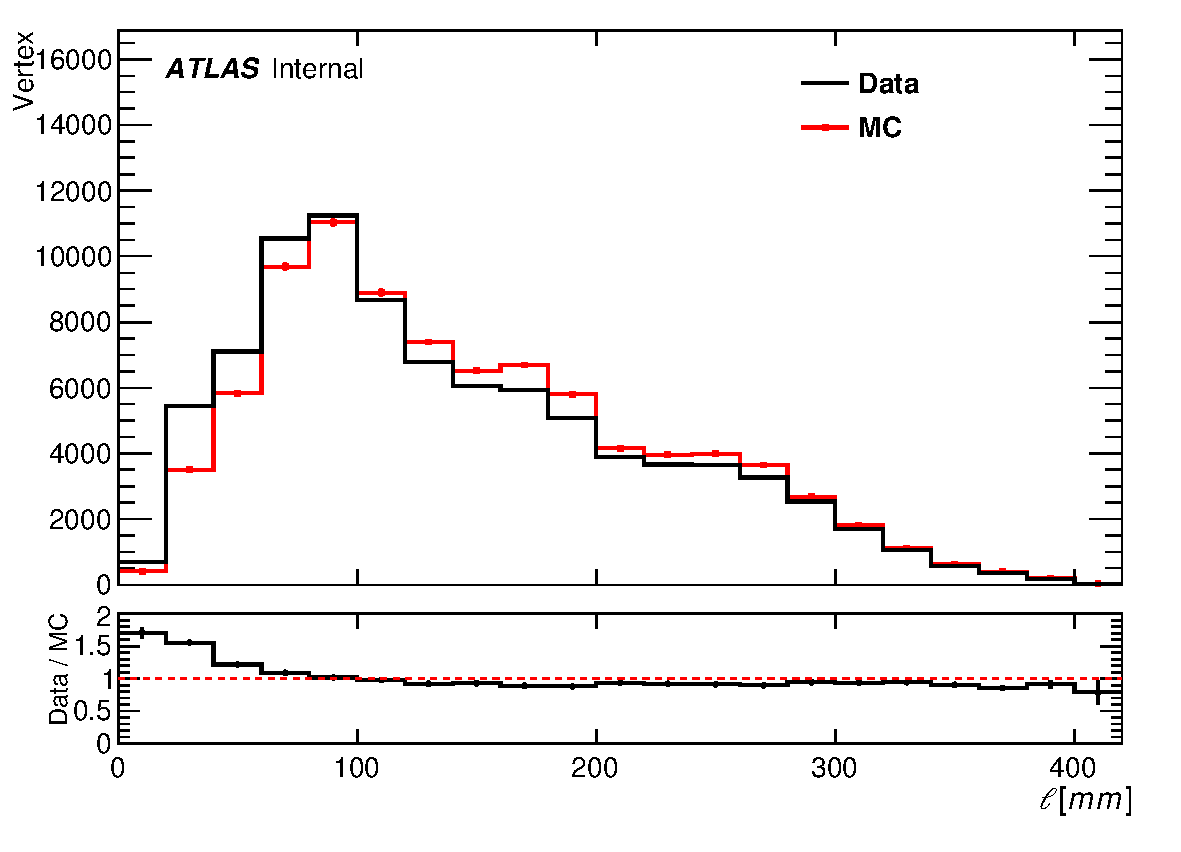
\includegraphics[width=0.45\textwidth]{figures/m_syst_Ks_l.pdf}} \\
    \caption{Comparison of the (a) invariant mass, (b) $p_{T}$, (c) $\mu$, (d) transverse, (e) longitudinal position, and (f) decay length of \Ks vertex with two large-radius tracks in the data with the MC samples. Data is normalized to MC. In (d), the red dashed lines indicate the four pixel layers and the first layer of SCT. The green dotted lines indicate the Inner Support Tube (45.5 mm) and Pixel Support Tube (229 mm). MC sample is reweighted to the pile-up distribution in data.}
    \label{fig:Ks_data_MC}
\end{figure}

\Ks vertices found in the data and the MC samples are binned in decay radius, $r$, and the \Ks yields in each bin are estimated after subtracting the background contributions using side-bands (350 - 450, 550 - 650 GeV) in the invariant mass distribution. Figure~\ref{fig:Ks_mass} shows the mass distribution of \Ks vertex with two large-radius tracks from the data and the MC samples. The figure shows that backgrounds are small and uniform in the mass window, and the mass distributions are in good agreement between the data and the MC samples.

%\begin{figure}[tb]
\begin{figure}[!htb]
    \centering
    \subfloat[]{\label{subfig:Ks_mass1}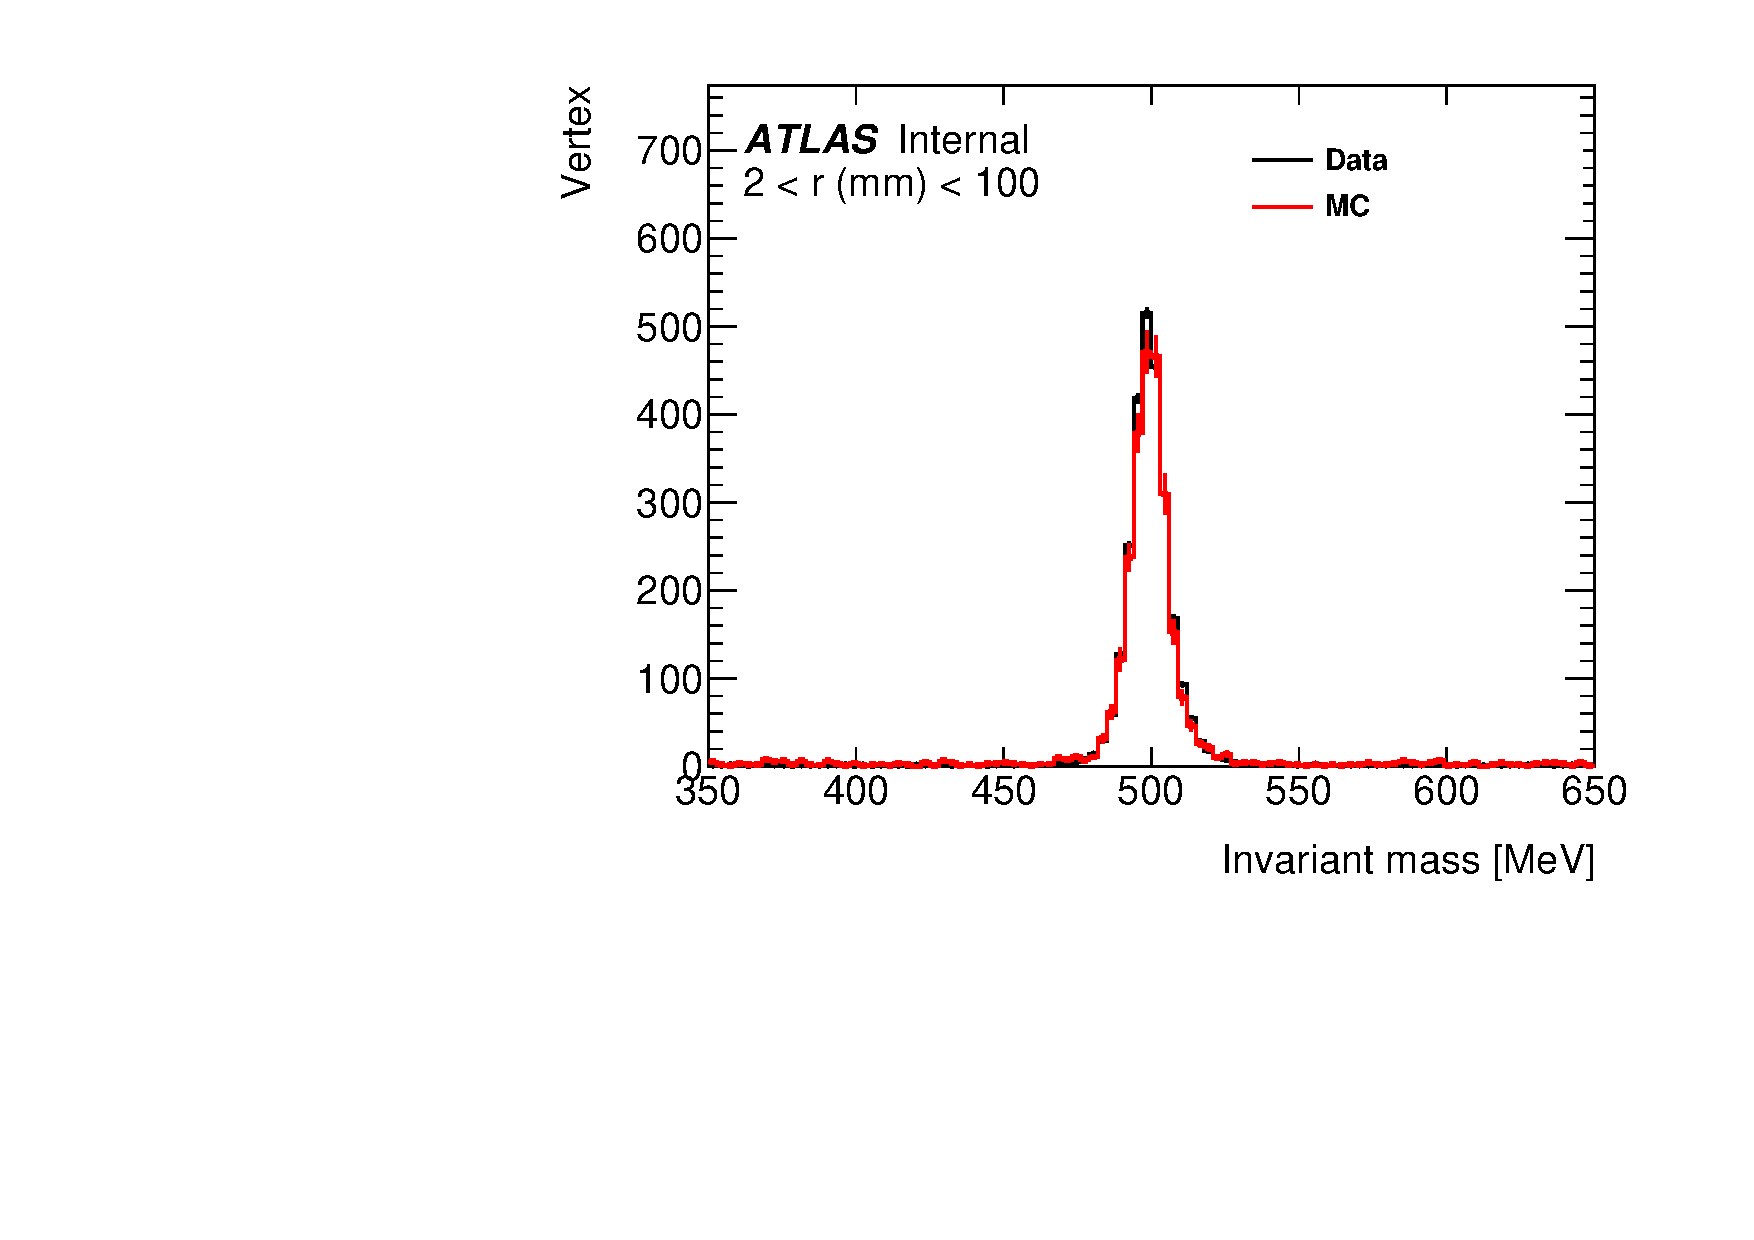
\includegraphics[width=0.50\textwidth]{figures/m_syst_Ks_normalized_LRT_R1.pdf}}
    \subfloat[]{\label{subfig:Ks_mass2}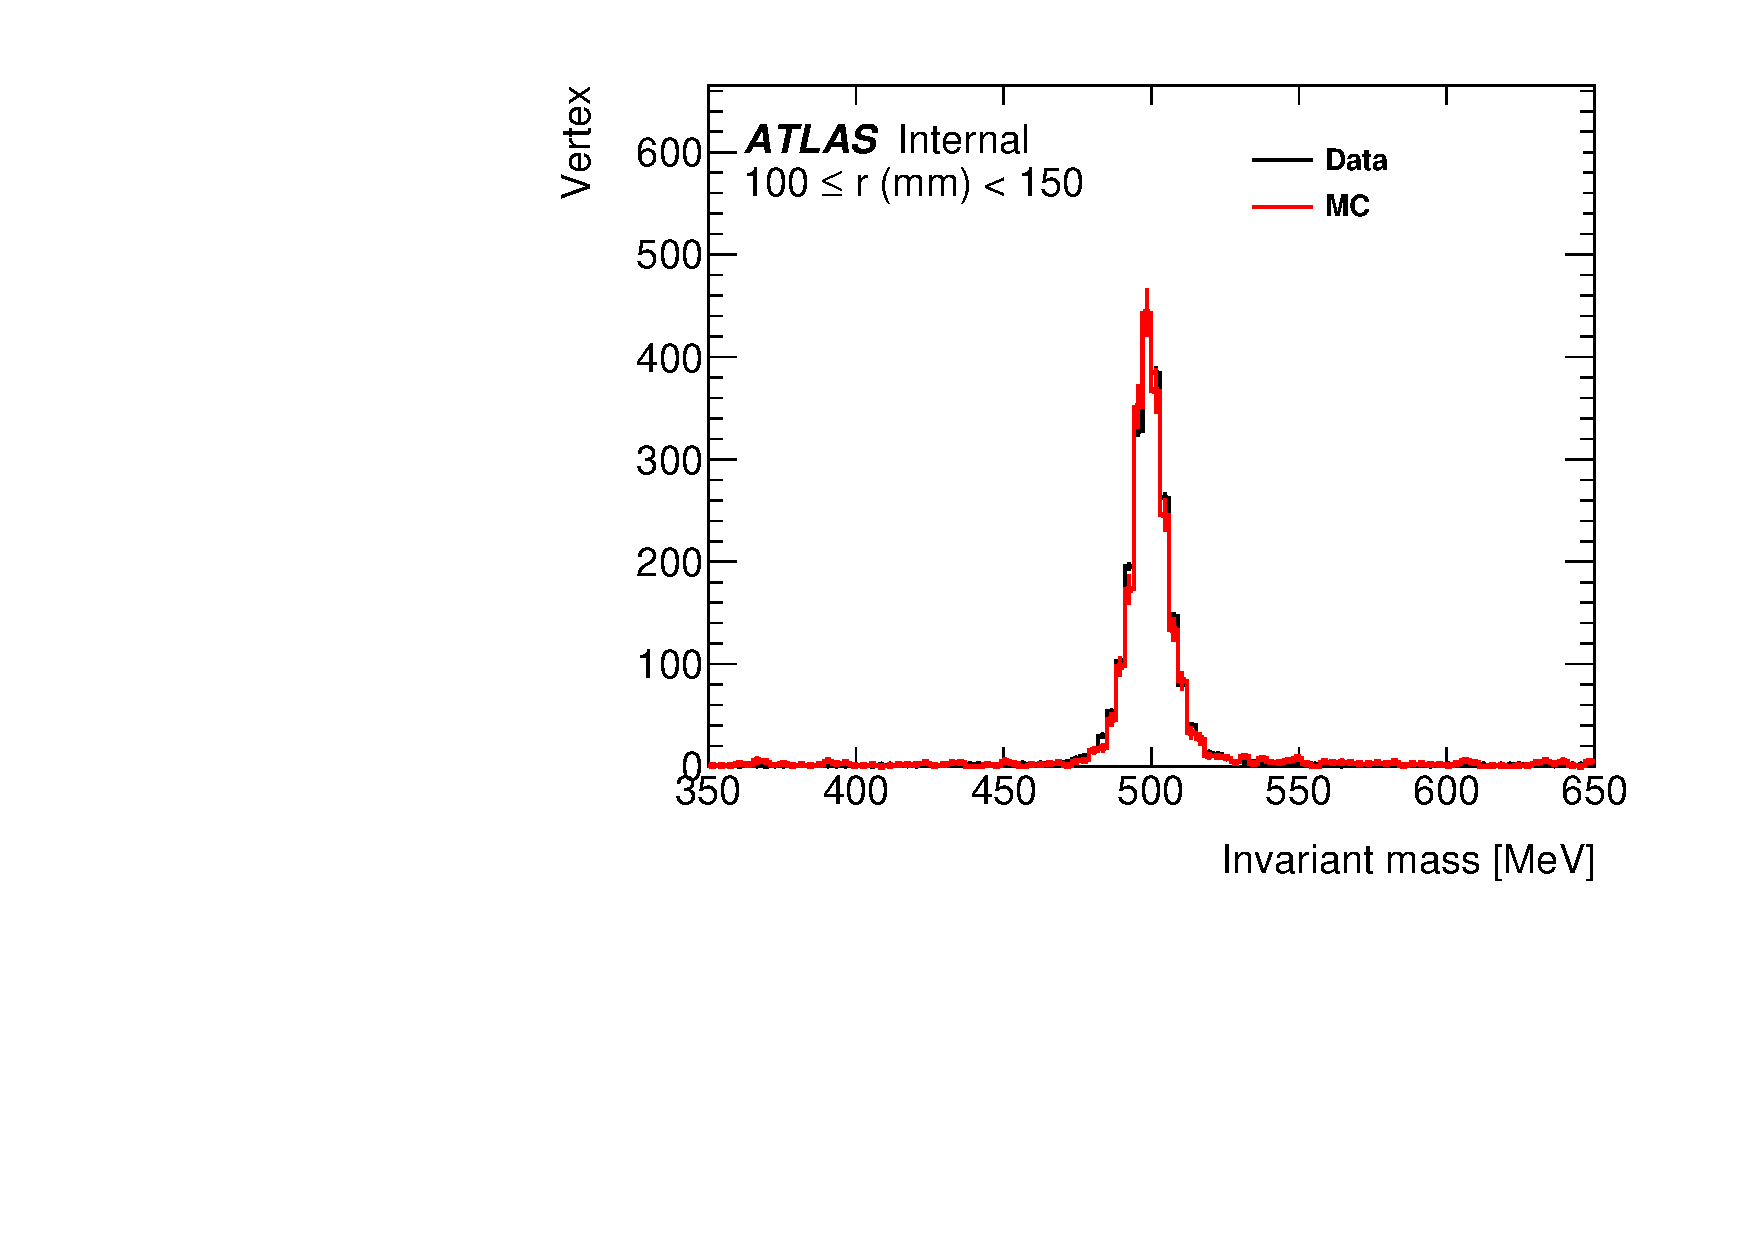
\includegraphics[width=0.50\textwidth]{figures/m_syst_Ks_normalized_LRT_R2.pdf}} \\
    \subfloat[]{\label{subfig:Ks_mass3}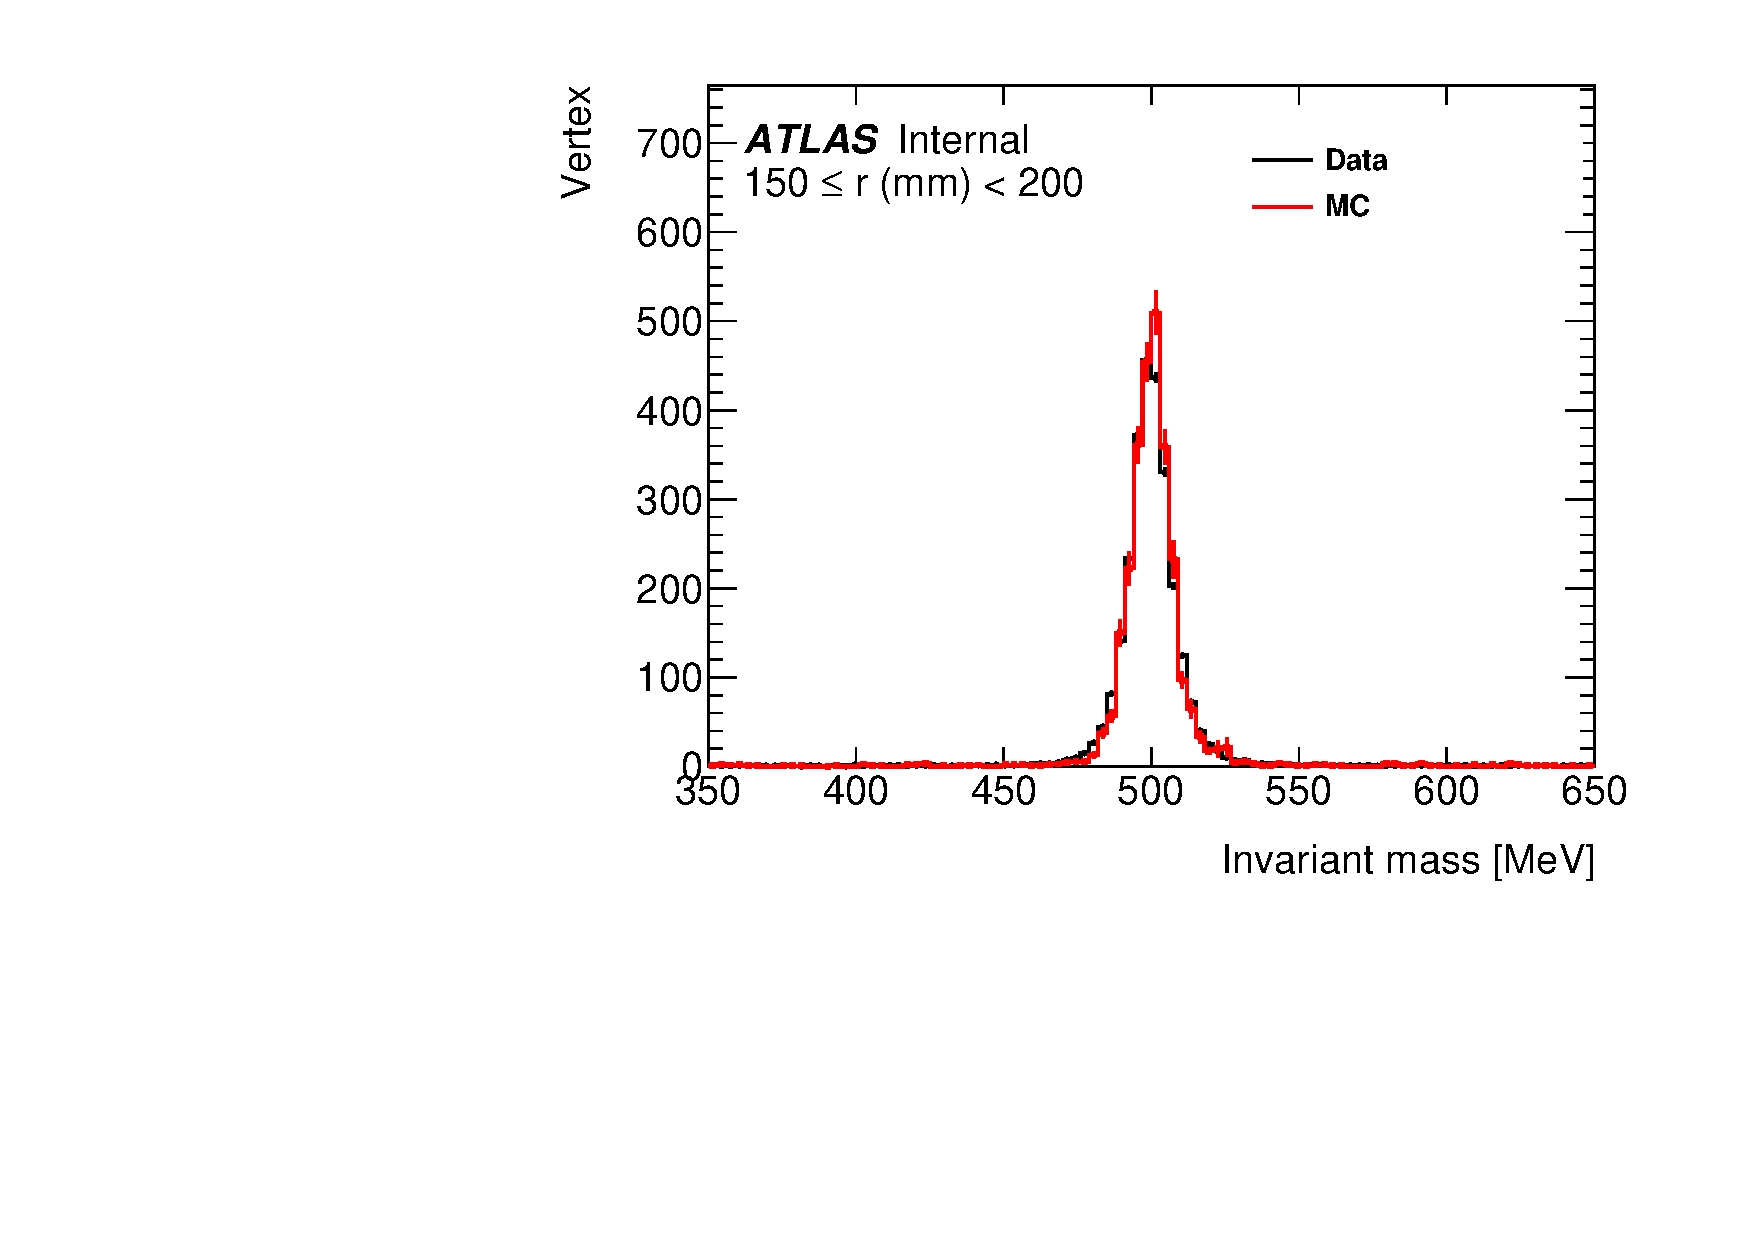
\includegraphics[width=0.50\textwidth]{figures/m_syst_Ks_normalized_LRT_R3.pdf}} 
    \subfloat[]{\label{subfig:Ks_mass4}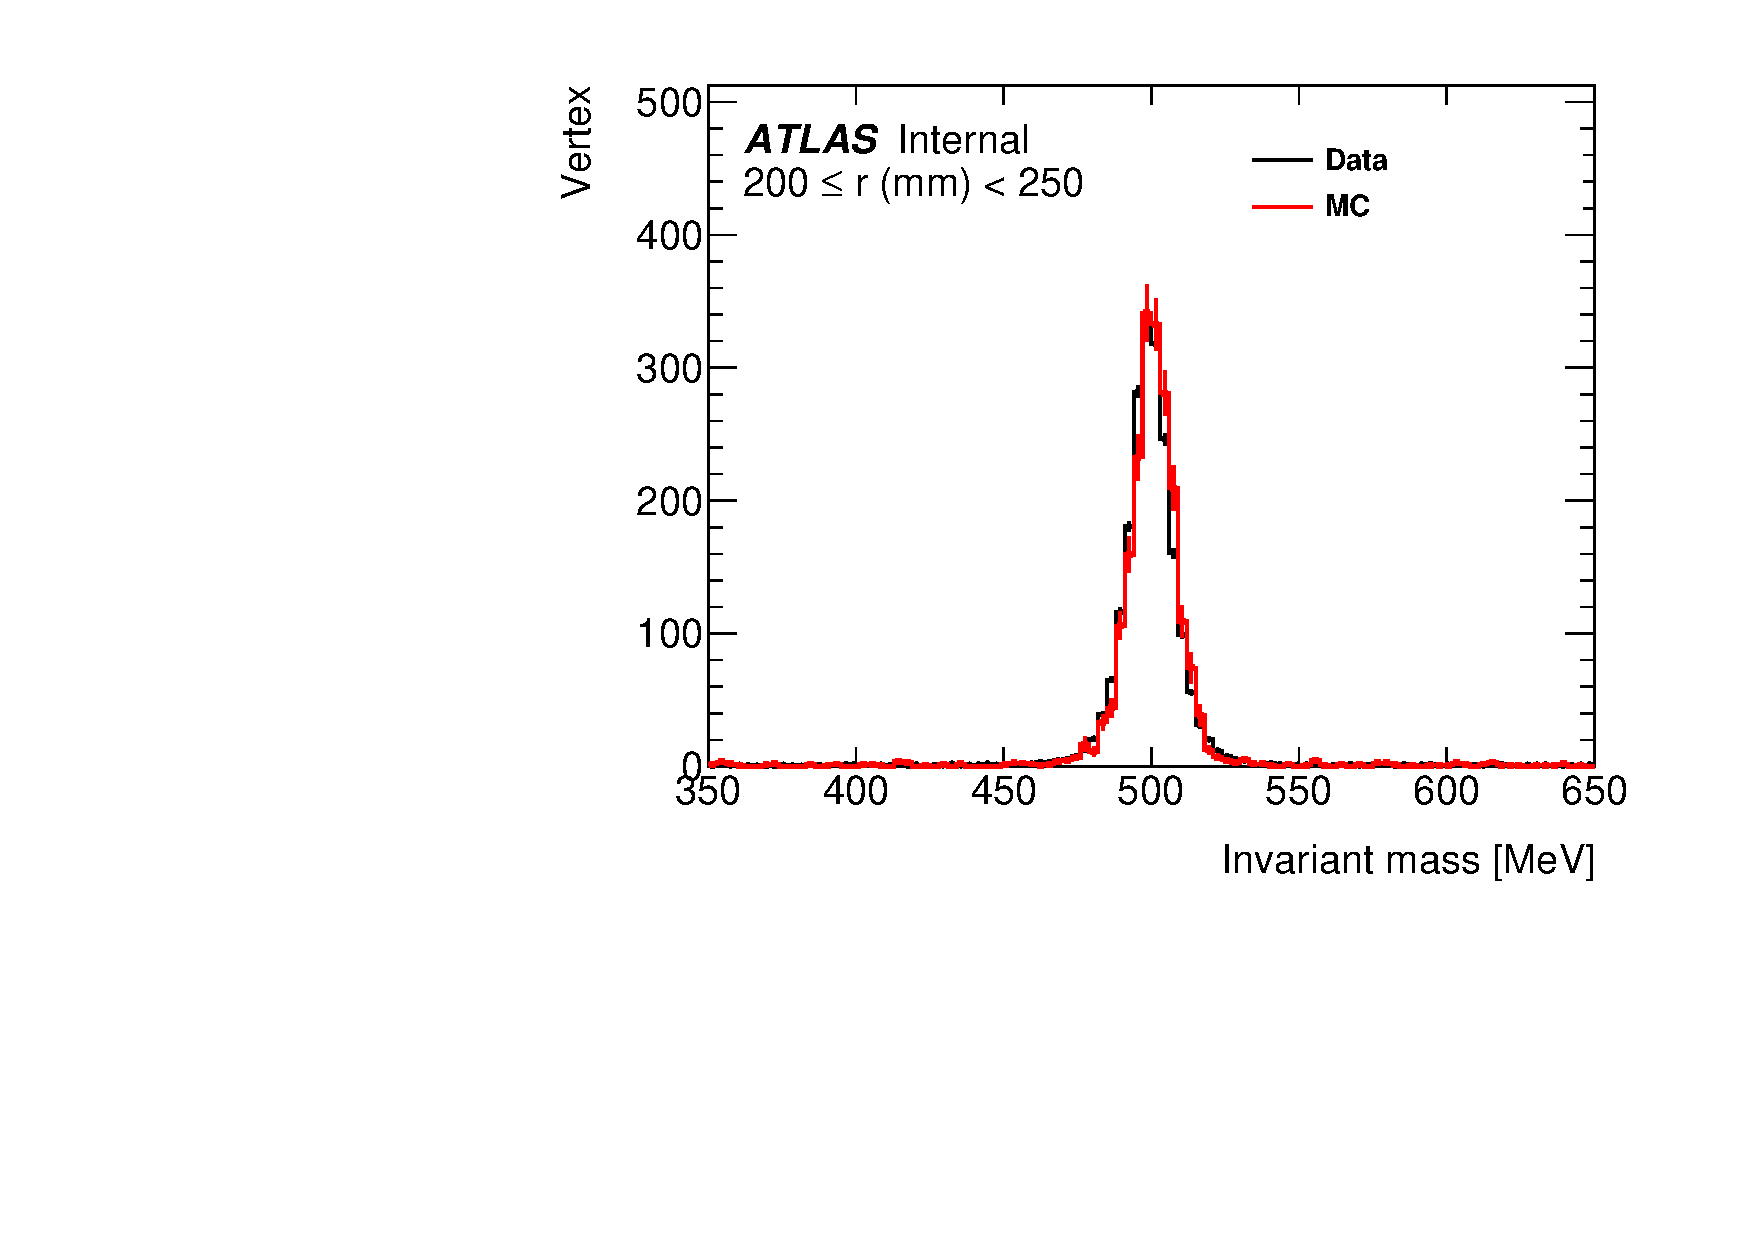
\includegraphics[width=0.50\textwidth]{figures/m_syst_Ks_normalized_LRT_R4.pdf}} \\
    \subfloat[]{\label{subfig:Ks_mass5}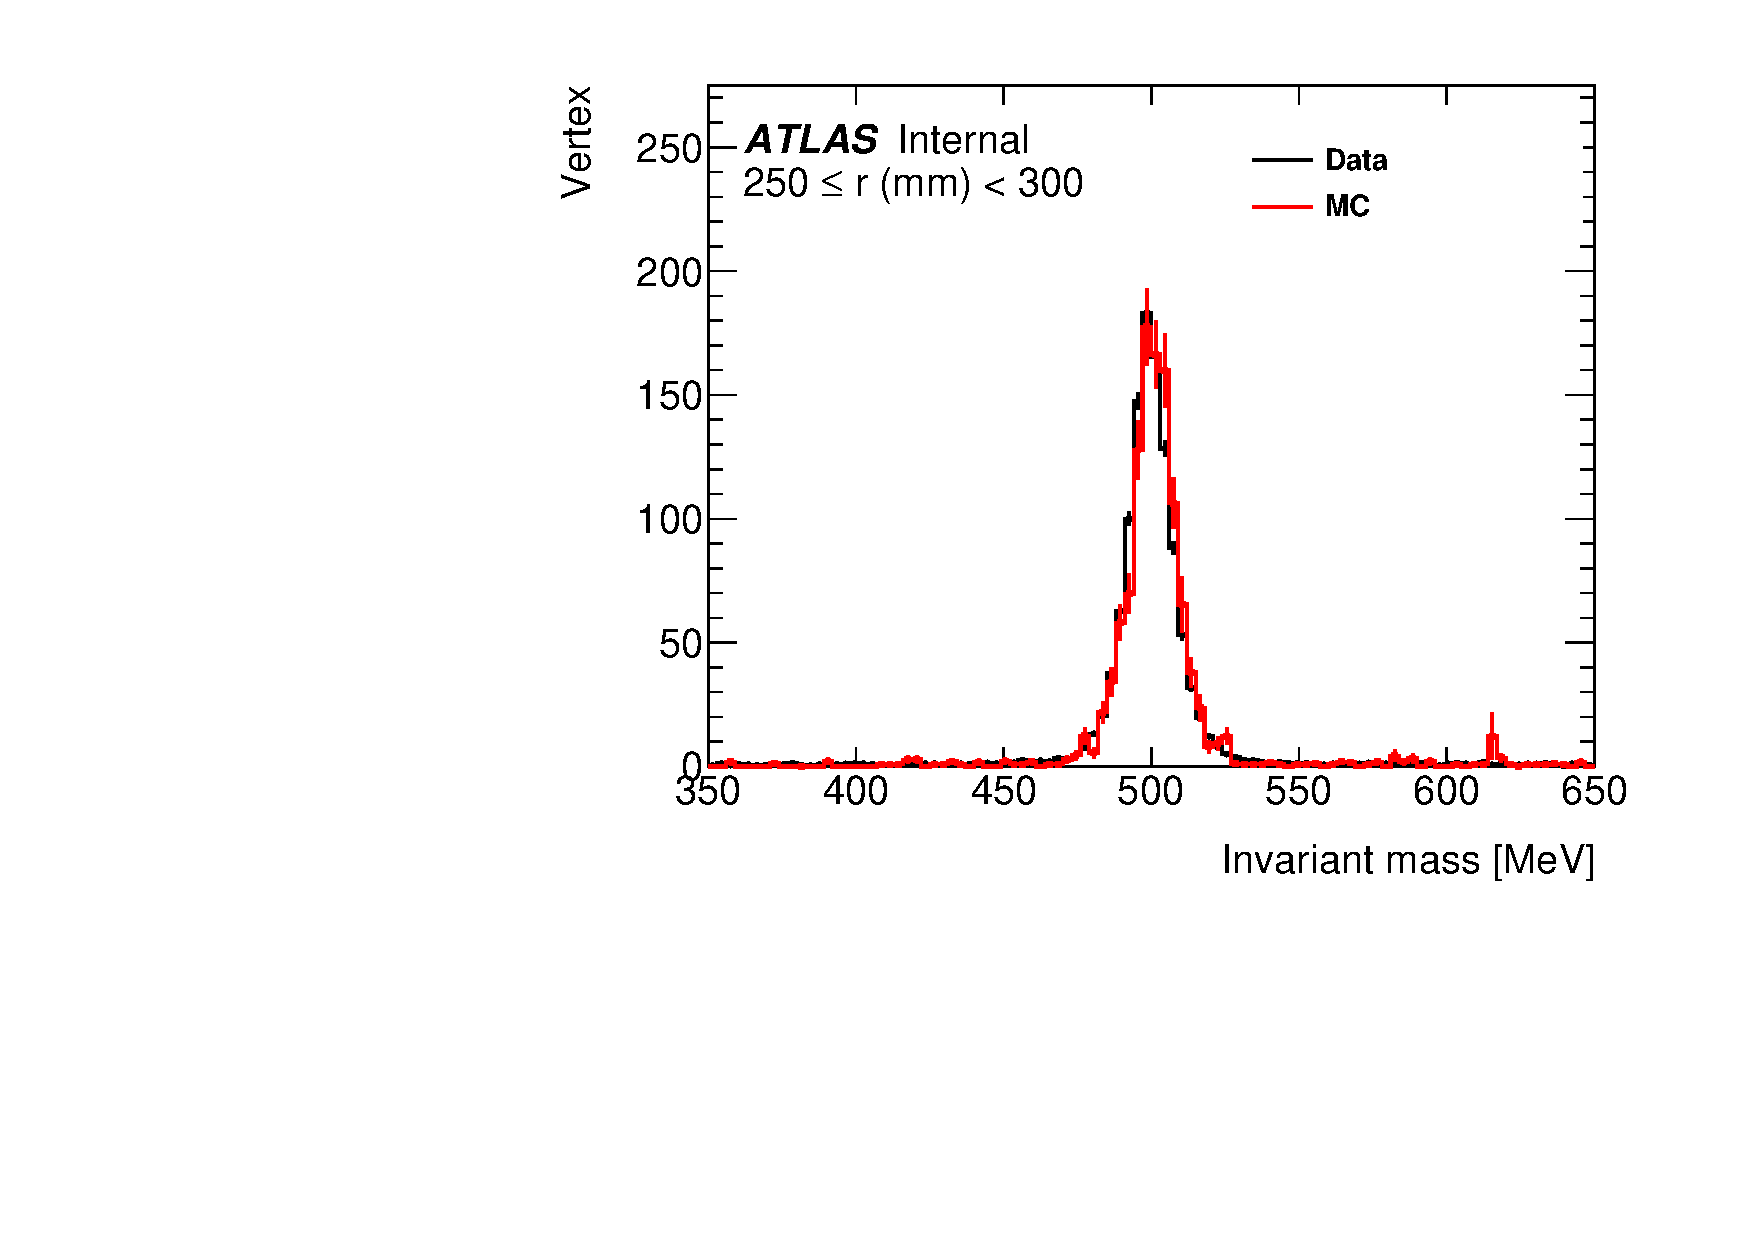
\includegraphics[width=0.50\textwidth]{figures/m_syst_Ks_normalized_LRT_R5.pdf}} 
    \caption{Representative distributions of the invariant mass of \Ks candidates with two large-radius tracks for (a) 2 < $r$ < 100 mm, (b) 100 $<r<$ 150 mm, (c) 150 $<r<$ 200 mm, (d) 200 $<r<$ 250 mm, and (e) 250 $<r<$ 300 mm in the data and the MC samples. Data is normalized to MC samples.}
    \label{fig:Ks_mass}
\end{figure}

The \Ks yields with two large-radius tracks are compared between data and MC samples in Figure~\ref{fig:Ks_double_ratio}, where the data is normalized by a factor of $N_{\mathrm{ST}} / N_{\mathrm{ST}}^{\mathrm{MC}}$, integrated over $r$. The ratio between two, representing the double ratio (Eq.~\ref{eq:Ks_eq2}), is shown in the lower pane.

\begin{figure}[!htb]
	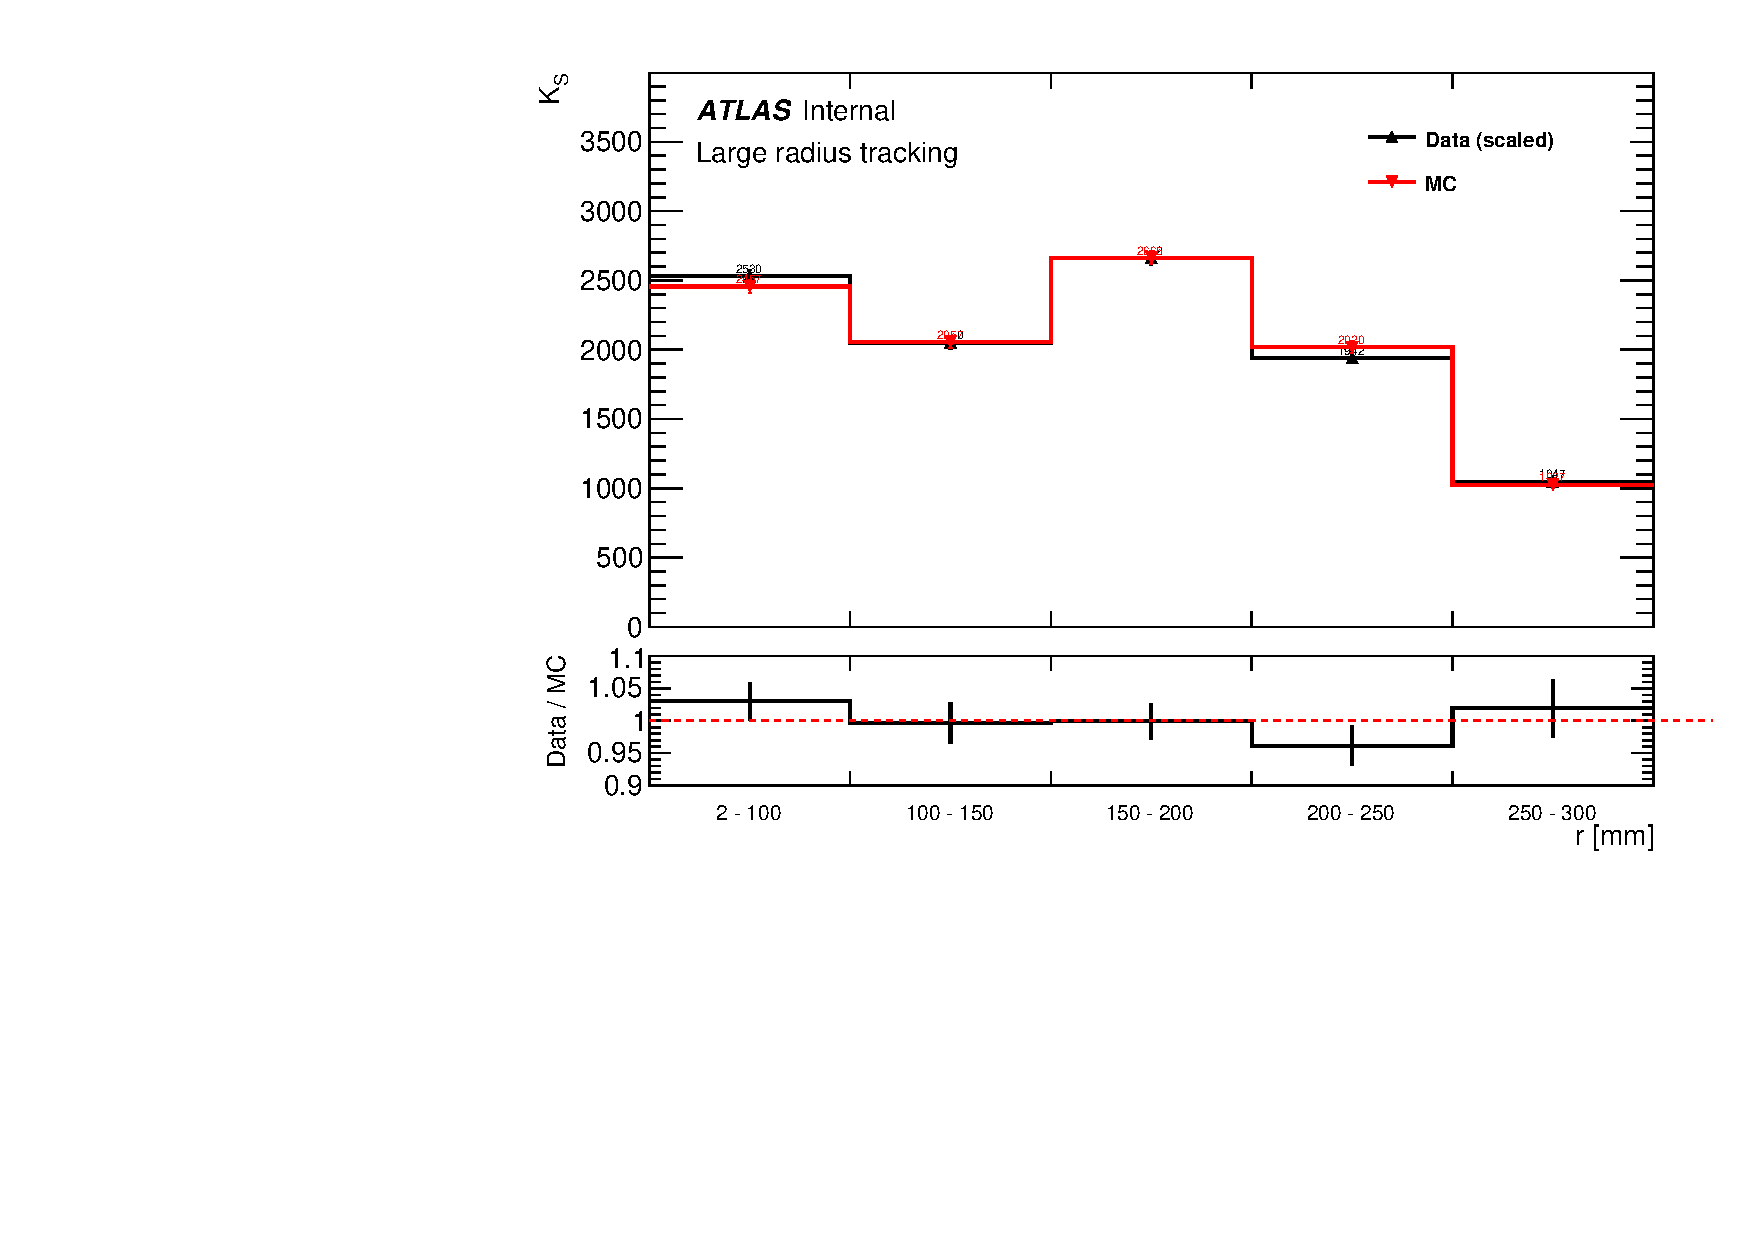
\includegraphics[width=0.70\textwidth]{figures/m_syst_Ks_ratio_LRT_R.pdf}
	\centering
	\caption{The radial distribution of \Ks yields with two large-radius tracks. Data is normalized to the MC for \Ks found with the ST tracking.} %The lower pane shows the double ratio defined in Eq.~\ref{eq:Ks_eq2}.}
	\label{fig:Ks_double_ratio}
\end{figure}

In estimating the systematic uncertainty, largest discrepancy ($4\%$), shown in the fourth bin, is taken as a conservative estimate of $(N_{\mathrm{LRT}} \cdot N_{\mathrm{ST}}^{\mathrm{MC}}) / (N_{\mathrm{LRT}}^{\mathrm{MC}} \cdot N_{\mathrm{ST}})$. The results from previous studies show that the systematic uncertainty in the standard tracking is $2\%$~\cite{ATL-PHYS-PUB-2015-051}, and the systematic uncertainty in secondary vertex reconstruction using standard tracks is $1\%$~\cite{Aaboud:2215485}. The study on secondary vertex reconstruction is performed using min-bias data, but relatively uniform distribution of efficiency as a function of pile-up (Figure~\ref{subfig:vertex_dist_mu}) suggests that this result is still applicable for data with $\langle \mu \rangle\approx$ 24. Using Eq.~\ref{eq:Ks_eq3} together with these results, the systematic uncertainty in track and vertex reconstruction in the LRT is estimated to be $10\%$\footnote{10\% is a conservative estimate of the calculation, $1.04\cdot1.02^{2}\cdot1.01\approx1.09$}.


%\subsection{Systematic uncertainty in Trigger Efficiency}
%\label{sec:syst_trigger}
%
%The efficiencies of all analysis triggers have been measured with tag-and-probe studies on data and MC as reported in Section~\ref{sec:trigger_efficiency}. Systematic uncertainties of tag-and-probe methods on the plateau efficiencies are usually of the order one percent and, therefore, negligible compared to other sources like tracking and vertexing. For this reason, no attempt was made to estimate systematic uncertainty in trigger efficiency.
%
%

\subsection{Systematic uncertainties on background estimations}
\label{sec:syst_bkg}

There are two main sources of background in this analysis; cosmic muon background and random crossing background. The cosmic muon background estimation is outlined in Section~\ref{sec:bkg:cosmic}. From this technique the estimate is $0.27 \pm 0.14 \textrm{ (stat.)}$ events. This $\pm 0.14$ is taken to be the total uncertainty on this background. In the case of the random crossing, there are two estimates event mixing and track flipping giving $2.40\times10^{-3}$ and $3.95 \times 10^{-3}$ respectively. For these the larger estimate of $3.95 \times 10^{-3}$ is used as the central value and the difference of $1.5\times10^{-3}$ is used as the uncertainty on this value.










